\documentclass[11pt]{article}
\usepackage[margin=1in]{geometry}                % See geometry.pdf to learn the layout options. There are lots.
\geometry{letterpaper}                   % ... or a4paper or a5paper or ... 
%\geometry{landscape}                % Activate for for rotated page geometry
%\usepackage[parfill]{parskip}    % Activate to begin paragraphs with an empty line rather than an indent
\usepackage[breaklinks=true, colorlinks=true, linkcolor=red, urlcolor=blue, citecolor=black]{hyperref}
\urlstyle{rm}
\usepackage{mathptmx}
\usepackage{graphicx}
\usepackage{amssymb}
\usepackage{epstopdf}
\usepackage{color}
\usepackage{sidecap}
\usepackage{authblk}
\usepackage{booktabs}
\usepackage[font=small,labelfont=bf]{caption}
\usepackage{enumitem}
\usepackage{wrapfig}
\DeclareGraphicsRule{.tif}{png}{.png}{`convert #1 `dirname #1`/`basename #1 .tif`.png}

\pagestyle{plain}

\def\bfr{\bf\color{red}}
\def\geohub{{\tt geohub}}
\def\resp{respectively}
\def\selah{SELAH}

%\title{\bf
%	Summary of SELAH Unsheltered Tract Recounts around\\ Echo Park Lake
%	}
%\author{}%,$\ddagger$
%
%\date{\today}                                           % Activate to display a given date or no date

\begin{document}
%\maketitle

\begin{center}
	\Large\bf Unsheltered Homelessness in Hollywood is Down\\
	\vspace{1ex}
	{\normalsize\rm Louis Abramson, PhD, and Brian Kohan 
	for the \href{http://www.hollywood4wrd.live}{\it Hollywood4WRD Coalition} \\ \today}

%	\vspace{1em}

%	{\large\it Summary}	
\end{center}

\noindent {\bf Summary:} The total number of people experiencing unsheltered homelessness in both the 
Hollywood and East Hollywood Communities has fallen since the last LAHSA Point-In-Time (PIT) 
estimate in January 2020. Based on data from the night of 25 February 2021, assuming no changes in
dwelling occupancy, these CoCs have seen decreases of $12\%\pm9\%$ and $15\%\pm12\%$ (90\% CI), \resp. If 
potential changes to the average number of people living in tents are incorporated, 20\% declines in both 
CoCs are possible. {\bfr External data lead us to favor reduced tent-occupancy, but definitive statements will 
require additional studies.} 

A $\sim$30\% reduction in individuals seen on the street drives these declines, which are sufficient to 
significantly lower {\it raw counts} of people and dwellings compared to 2020 in 14 out of 39 US Census tracts. 
Meanwhile, only seven tracts saw significant increases, with makeshift dwellings the only category to increase in the 
past 13 months. These declines persist irrespective of counter (professional vs.\ volunteer), span coherent geographies 
surveyed by independent teams, and are larger than what can be accounted for data acquisition errors, alone. 
As such, the qualitative trend should not depend on demographic weighting factors. 

Instead, it may partially reflect a combination of COVID-related initiatives aimed at placing and keeping people in 
housing. Eviction moratoria may have reduced inflow while Project Roomkey, various emergency shelters, and the 
opening of at least one {\it A Bridge Home} site may have moved people indoors. As such, while the unsheltered 
fraction may have fallen, homelessness in toto may not have decreased in Hollywood. Moreover, given the closure
of many facilities used by unhoused people for basic functions, conditions for those remaining on the street may
have deteriorated markedly. Data from the Coordinated Entry System should constrain both possibilities.

\begin{figure*}[h]
	\centering
	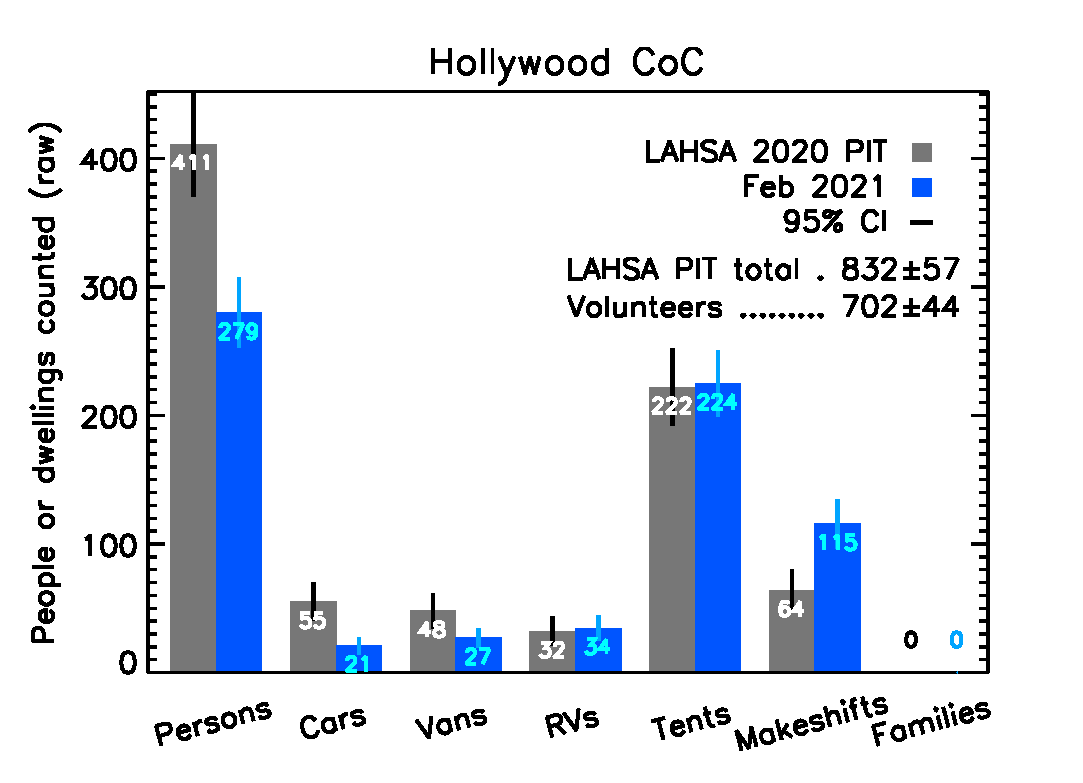
\includegraphics[width = 0.47\textwidth, trim = 1cm 0cm 0cm 0cm]{Hwood2021Bars}
	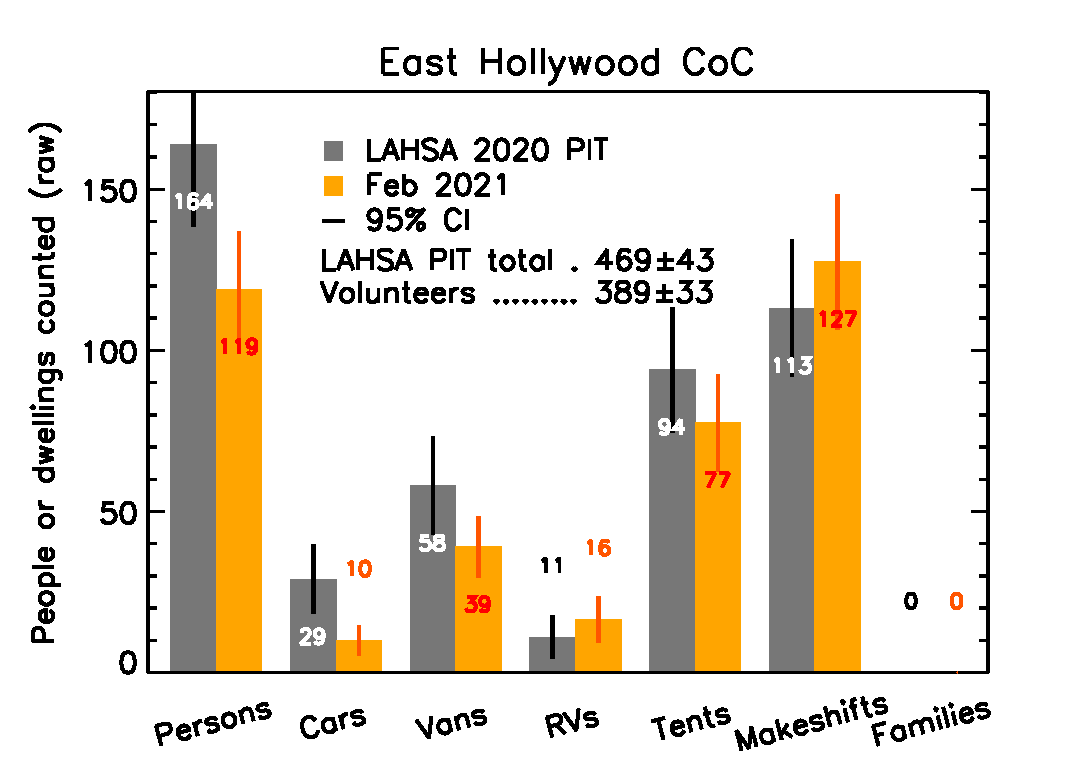
\includegraphics[width = 0.47\textwidth, trim = 1cm 0cm 0cm 0cm]{Eho2021Bars}
	\caption{}
	\label{fig:rawCounts}
\end{figure*}

\begin{figure*}[]
	\centering
	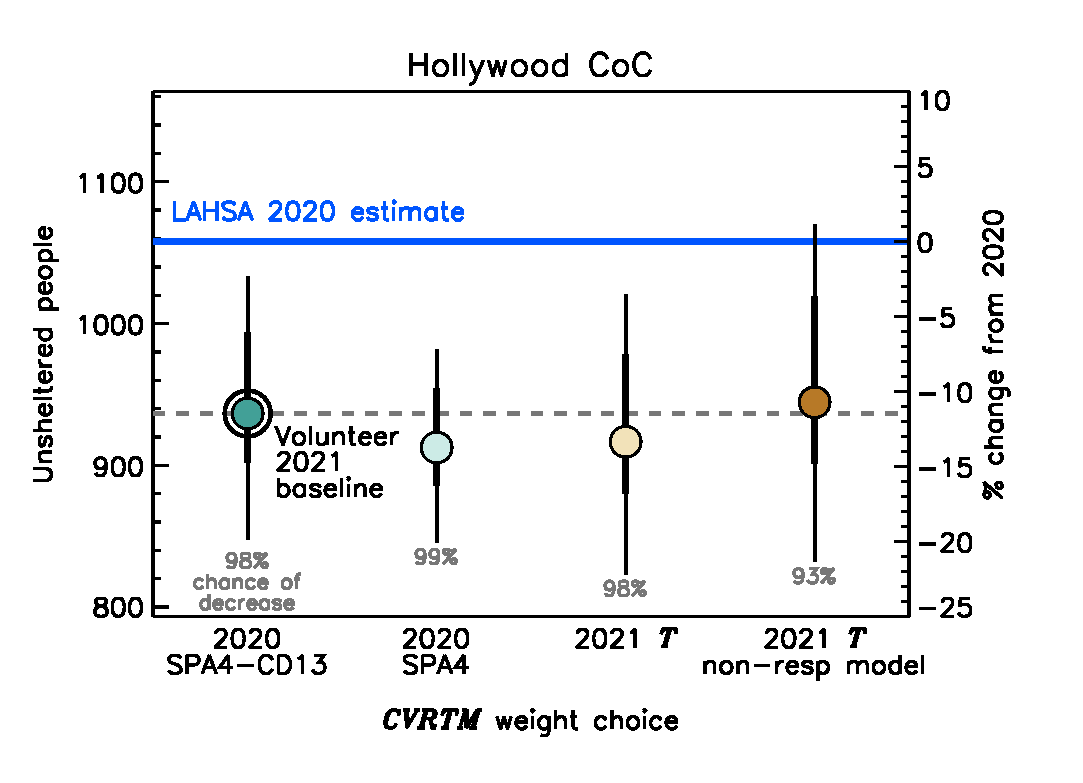
\includegraphics[width = 0.48\textwidth, trim = 1cm 0cm 0cm 1cm]{hwoodFinal}
	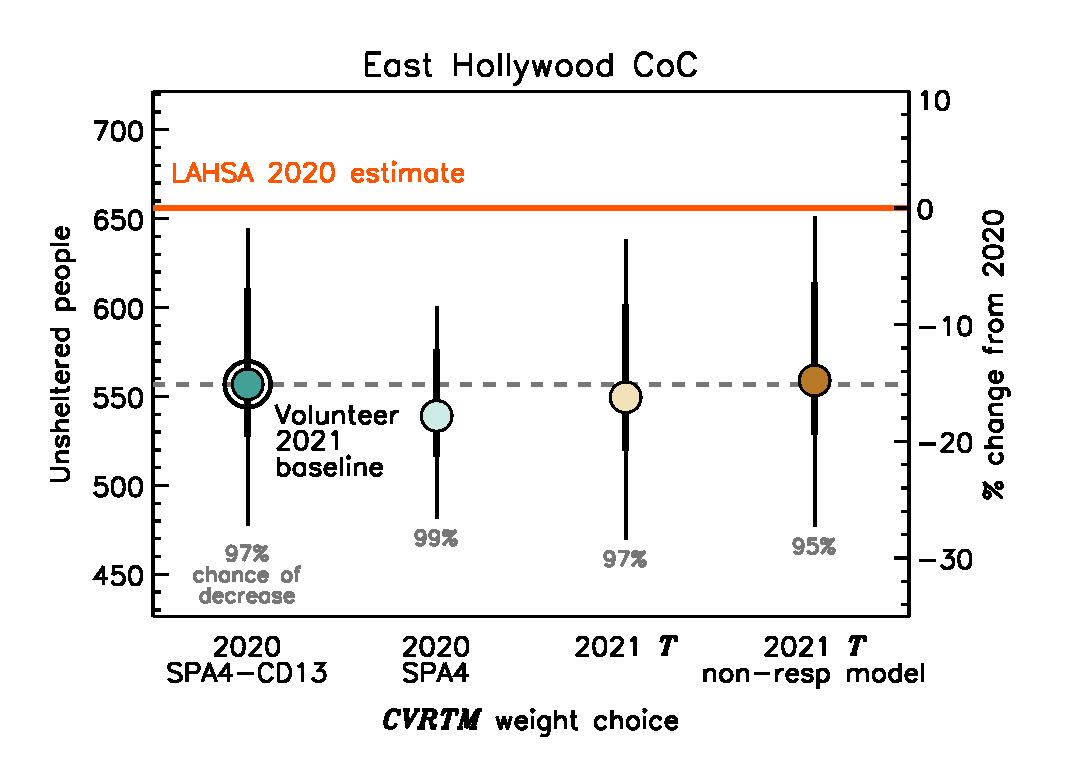
\includegraphics[width = 0.48\textwidth, trim = 1cm 0cm 0cm 1cm]{ehoFinal}
	\caption{}
	\label{fig:tcomp}
\end{figure*}

\begin{figure*}[]
	\centering
	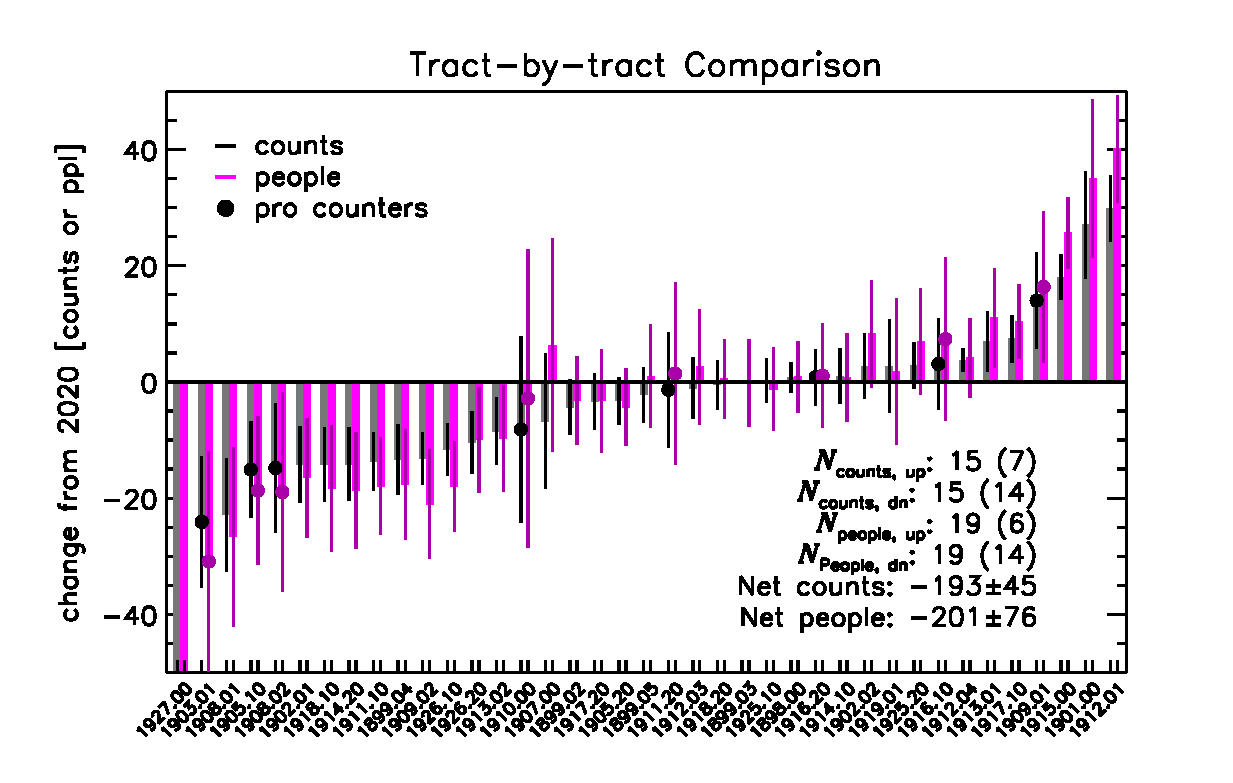
\includegraphics[width = \textwidth, trim = 0cm 0cm 0cm 0cm]{tractsYrYr}
	\caption{}
	\label{fig:tcomp}
\end{figure*}

\href{https://projectroomkeytracker.com/}{PRK Tracker; 1608 near night of count}
\href{https://www.lahsa.org/documents?id=4686-2020-greater-los-angeles-city-community-homelessness-report-service-planning-area-4.pdf}{LAHSA stats from this report}

{\bfr If Hwood and Eho's share of total LACo unsheltered homelessness are good proxies, something
like 60 formerly unsheltered ppl may have been in Roomkey the night of the count (1608 occupied rooms). 
Unclear how much of this was for folks in ABH, which would not reflect a net increase of sheltered ppl.}

%\begin{table*}[h]
%\caption{Hollywood CoC Unsheltered Data}
%\resizebox{\linewidth}{!}{%
%\begin{tabular}{lccccccccccc}
%\toprule
% & Adult & TAY & Unacc Minor & Car & Van & RV & Tent & Makeshift & Family & {\bf 2021 Total} & {\bf 2020 Total} \\ \cmidrule{1-12}
%{\bf Hollywood} \\ %\cmidrule{1-1}
%Counts & 277 & 2 & 0 & 21 & 27 & 34 & 224 & 115 & 0 & {\bf 702} & {\bf 831} \\
%Inhabitants & 277 (27) & 2 (5) & 0 (3) & 32 (11) & 49 (13) & 50 (14) & 332 (29) & 195 (24) & 0 (3) & {\bf 937 (93)} & {\bf 1058} \\% (76)
%Category share & 0.30 (0.03) & 0.00 (0.00) & 0.00 (0.00) & 0.03 (0.01) & 0.05 (0.01) & 0.05 (0.01) & 0.35 (0.03) & 0.21 (0.03) & 0.00 (0.00) & -- & -- \\ \cmidrule{1-12}
%{\bf East Hollywood} \\ %\cmidrule{1-1}
%Counts & 114 & 4 & 0 & 10 & 39 & 16 & 77 & 127 & 0 & {\bf 389} & {\bf 469} \\
%Inhabitants & 114 (19) & 4 (4) & 0 (3) & 15 (8) & 70 (15) & 24 (9) & 115 (19) & 216 (23) & 0 (3) & {\bf 557 (83)} & {\bf 656} \\% (60)
%Category share & 0.20 (0.03) & 0.01 (0.01) & 0.00 (0.00) & 0.03 (0.01) & 0.13 (0.03) & 0.04 (0.02) & 0.20 (0.03) & 0.39 (0.04) & 0.00 (0.00) & -- & --
%\\ \bottomrule
%\end{tabular}
%}
%\caption*{Quantities in parentheses denote 95\% uncertainties (binomial in the case of the categories). Uncertainties larger than estimates imply that only upper limits can be stated confidently.}
%\label{tbl:}
%\end{table*}

\begin{table*}[h]
\caption{Hollywood CoC Unsheltered Data}
\resizebox{\linewidth}{!}{%
\begin{tabular}{lcccccccccc}
\toprule
 & Adult & TAY & Car & Van & RV & Tent & Makeshift & {\bf 2021 Total} & {\bf 2020 Total} & Difference \\ \cmidrule{1-11}
{\bf Hollywood} \\ %\cmidrule{1-1}
Counts & 277 & 2 & 21 & 27 & 34 & 224 & 115 & {\bf 702} & {\bf 831} & $-129$ \\
Inhabitants & 277 (27) & 2 (5) & 32 (11) & 49 (13) & 50 (14) & 332 (29) & 195 (24) & {\bf 937 (93)} & {\bf 1058} & $-121$ (93)\\% (76)
Category share & 0.30 (0.03) & 0.00 (0.00) & 0.03 (0.01) & 0.05 (0.01) & 0.05 (0.01) & 0.35 (0.03) & 0.21 (0.03) & -- & -- & -- \\ \cmidrule{1-11}
{\bf East Hollywood} \\ %\cmidrule{1-1}
Counts & 114 & 4 & 10 & 39 & 16 & 77 & 127 & {\bf 389} & {\bf 469} & $-80$ \\
Inhabitants & 114 (19) & 4 (4) & 15 (8) & 70 (15) & 24 (9) & 115 (19) & 216 (23) & {\bf 557 (83)} & {\bf 656} & $-99$ (83)\\% (60)
Category share & 0.20 (0.03) & 0.01 (0.01) & 0.03 (0.01) & 0.13 (0.03) & 0.04 (0.02) & 0.20 (0.03) & 0.39 (0.04) & -- & -- &--
\\ \bottomrule
\end{tabular}
}
\caption*{Quantities in parentheses denote 95\% uncertainties (binomial in the case of the categories). Uncertainties larger than estimates imply that only upper limits can be stated confidently.}
\label{tbl:}
\end{table*}


\clearpage

%\begin{wrapfigure}{r}{0.5\linewidth}
%	\centering
%	\includegraphics[width=\linewidth]{t1975}
%	\caption{US Census tract 1975.00.}
%	\label{fig:tract}
%\end{wrapfigure}
%\noindent {\bf Context:} \selah\ volunteers performed two recounts of US Census tract 1975.00 
%on 2 August and 18 October 2020 (Figure \ref{fig:tract}). This tract contains Echo Park Lake and various 
%CalTrans lands. The results of both surveys were statistically identical except for the estimate of vans, 
%which rose from $14\pm3$ to $25\pm5$ between counts. Our final individual/dwelling statistics 
%(Table \ref{tbl:rawData}) and total population estimates (Figure \ref{fig:results}) reflect the average 
%of those assessments.\\


\noindent {\bf Results and uncertainties:} The population inferences in Figure \ref{fig:results} come 
from 10,000 Monte Carlo resamplings of the \selah\ survey data with counts perturbed by random 
draws from their Poisson error bars. In the cases of cars, vans, RVs, tents, and makeshift (CVRTM) 
dwellings, we additionally boosted counts by the relevant weighting factor perturbed by its error bar. 
In the baseline case---shown as blue horizontal bands in Figure \ref{fig:results}---we use the official 2020 
\href{https://www.lahsa.org/documents?id=4693-2020-greater-los-angeles-homeless-count-cvrtm-conversion-factors}{LAHSA SPA4 CVRTM weights}. The median result of that inference yields $220\pm30$ unsheltered 
individuals (90\% CI) compared to the PIT's estimate of 174 people.\\
\indent The CVRTM weights present systematic uncertainties, however, and so possible biases. 
For example, service providers have made a concerted effort to distribute tents during COVID, 
which might modulate $T$ downwards. (Other weights may have also shifted, but the fraction of 
tent-dwelling is such that changes to $T$ dominate the measurement error.) As such, multiplying by the 
2020 LAHSA tent weight may result in an overestimate of the actual unsheltered population.\\
\indent \selah\ cannot re-measure $T$ on large geographies, but two small-scale estimates 
suggest it has indeed fallen from the official 2020 value of 1.45 people per tent:
\begin{enumerate}
	\item \selah\ outreach teams surveyed 30 tents along Echo Park Lake's southern border on 21 
	February 2021, finding 11 of them to be used for storage or---based on statements from 
	neighbors or the team's weekly experience---abandoned. Albeit small, this sampling suggests that 
	up to 28\%--45\% of tents may be uninhabited (95\% CI) effectively reducing $T$ to 0.9.\footnote{
	Note: the official CVRTM weights are established using a 
	\href{https://www.lahsa.org/documents?id=4658-usc-2020-homeless-count-methodology-report}{methodology} that may not account for empty tents, and therefore may generally lead to overestimates of
	some degree.}
	\item Business Improvement District surveys of Hollywood conducted biweekly since January 2020 
	show the number of tents to have risen there faster than the number of visible individuals. Those
	data imply an average tent occupancy of $T=1.1\pm0.07$ people today.
\end{enumerate}
\noindent Using the lower unoccupied tent fraction in (1) to allow for inhabitants simply not being home, both 
modifications reduce our median unsheltered estimate to about 190 people---16 more than the 2020 PIT value.

\indent In all cases, further rigorous surveys---especially those aimed at understanding the fraction of
tents not used as  dwellings---are needed to ensure we understand the current scale of the 
homelessness crisis and plan accordingly.

We attribute this phenomenon to a combination of government initiatives aimed at both moving unhoused
residents indoors---e.g., Project Roomkey---and keeping housed people in their homes---e.g., City and State
eviction moratoria. 


This decrease is seen in raw counts and inferred total
population, in tracts counted by volunteers and professionals, in adjacent geographies counted by independent
teams, and at a level that cannot be accounted for by data acquisition errors. Recent observations suggesting
reduced tent occupancies during COVID only exacerbate the decline, which can be reversed only by assuming
a failure to count cars and vans used as dwellings that is not supported by cross-counter comparisons.




However, while the numbers may have declined since the onset of the pandemic, conditions on the street
have likely 

\end{document}  